\section{Plato parabólico}
\label{sec:plato}

\begin{problem}
Simule un plato parabólico en SolTrace que tenga un ángulo de borde $\psi_b = \pi/2$ y una apertura de dos metros.  
\end{problem}



\TheSolution Primero, considerese la parábola de la Figura~\ref{fig:parabola} generada con la con la ecuación~\eqref{eq:parabola} definida por el foco $f$.

\begin{equation}
  \label{eq:parabola}
  y = \dfrac{x^2}{4f} -f
\end{equation}


\begin{figure}[ht]
  \centering
  \subfigure[]{
    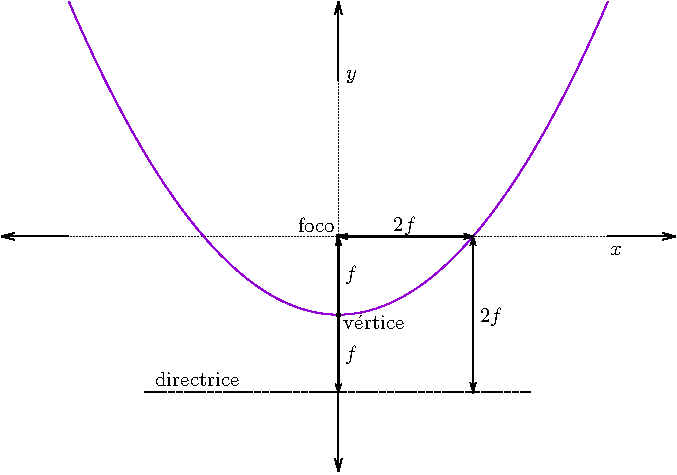
\includegraphics[width=0.45\textwidth]{figures/parabola}}
  \subfigure[]{
    \includegraphics[width=0.45\textwidth]{figures/parabolaPolares}}
  \caption{\label{fig:parabola} Parábola con el foco en el origen.}
\end{figure}

Es decir, que si el ángulo de borde es de $\pi/2$, implica que $x_b=1$~m ya que la apertura es de dos metros y entonces $f$ es de 0.5~m.

Sabemos\cite{Rabl1985active} que para un receptor cilíndrico el diámetro del receptor esta dado por la ecuación~\eqref{eq:diametro}. Si consideramos que el semi-ángulo de aceptación $\Delta_r$ es del tamaño del cono solar, entonces $\Delta = $4.65~mrad. Luego entonces podemos calcular el diámetro del receptor ideal y es igual 9.3~mm.



\begin{equation}
  \label{eq:diametro}
  D = \dfrac{4 \Delta_r f}{1 + \cos \psi_b}
\end{equation}

\ASolution Para simular este disco parábolico consideraremos un vector solar paralelo al eje $z$, es decir $\hat s = (0, 0, 1)$ y una forma Gaussiana. Respecto a los paramámetros ópticos, para el concentrador consideraremos una reflectividad casi especular de 0.96, una transmitancia de practicamente cero, sin errores de pendiente y especularidad. La Tabla~\ref{tab:opticaDisco} muestra los parámetros mencionados. Para el receptor generamos otro elemento en donde la reflectancia será nula.

\begin{table}[h]
  \centering
  \begin{tabular}[h]{ccccc}
    \toprule
    Reflectivity & Transmissivity & Slope error & Specularity error & Error type\\
    \midrule
    0.96         & 0.0001         & 0.0001      & 0.0001            & Gaussian\\
    \bottomrule
  \end{tabular}
  \caption{\label{tab:opticaDisco} Propiedades ópticas}
\end{table}

En la sección de etapas vamos agenerar nuevamente dos elementos, una para el concentrador y una para el receptor. La Tabla~\ref{tab:etapaReceptorD} muestra los parámetros del concentrador, para lo cual es necesario primero, mediante el boton \emph{Insert}, insertar un elemento. En el cual ingresaremos la posición del paraboloide, que sera el origen, en donde la su normal coincide con el \emph{aimpoint} es decir $(0, 0, 1)$. La apertura es circular con un diámetro de 2~m y el tipo de superficie es una parabóla con un foco de $f = 0.5$~m. El tipo de interacción es \emph{Reflection} y en el elemento \emph{Optics} seleccionamos el de \emph{concentrador} que previamente habíamos definido.

\begin{table}[h]
  \centering
  \scriptsize
  \begin{tabular}[h]{lllllllll}
    \toprule
    X-C & Y-C & Z-C & X-AimP & Y-AimP & Z-AimP & Z-Rot & Aperture & Surface\\
    \midrule
    0 & 0 & 0 & 0 & 0 & 1 & 0 & c-2,0,0,0,0,0,0,0 & p-1,1,0,0,0,0,0,0\\
    \bottomrule
  \end{tabular}
  \caption{\label{tab:etapaReceptorD} Etapa del concentrador.}
\end{table}

En la segunda etapa generamos el receptor circular plano posicionado en el foco, es decir, úbucado en $(0, 0, 0.5)$, y con un \emph{aimpoint} de $(0, 0, -1)$ sigue siendo paralelo al eje $z$ pero en sentido contrario. Seguimos teniendo una apertura circular con el radio calculado de 9.3~mm, pero ahora tenemos una superficie plana. Ahora las propiedades ópticas seran las definidas como \emph{concentrador}.

\begin{table}[h]
  \centering
  \scriptsize
  \begin{tabular}[h]{lllllllll}
    \toprule
    X-C & Y-C & Z-C & X-AimP & Y-AimP & Z-AimP & Z-Rot & Aperture & Surface\\
    \midrule
    0 & 0 & 0.5 & 0 & 0 & -1 & 0 & c-0.0093,0,0,0,0,0,0,0 & f-0,0,0,0,0,0,0,0\\
    \bottomrule
  \end{tabular}
  \caption{\label{tab:etapaReceptorR} Etapa del receptor }
\end{table}

Ya que tenemos de finido el sistema podemos proceder a realizar la simulación, para lo cual seleccionaremos 1,000,000 de rayos. Una vez indicado el numero de rayos procedemos a realizar la simulación mediante el botón \emph{Start new trace}.

La sección de \textbf{Results} tiene tres secciones: \emph{Intersections}, \emph{Flux Maps} y \emph{Ray Data}. En la sección de \emph{Intersections} podemos visualizar los distintos elementos simulados, en donde solo observaremos la interacción de los rayos con las superficies si existen, también tenemos la opción de imprimir la trayectoria de los rayos deseados.

La Figura~\ref{fig:inter} muestra la sección de \emph{Intersections} en ella podemos seleccionar la etapa de trazados de rayos y los elementos que contienen para visualizarlos. Una vez seleccionados se visualizan en la interacción de los rayos con las superficies que interactual, a demás si seleccionamos \emph{Plot path of ray \#s} podemos indicar el intervalo de rayos que deseamos visualizar. Los rayos que se muestran en color rojos son aquellos que no inciden en el receptor. En esta sección se indica cual es la irradiancia considerada para la simulación, en este caso es de 1,000 $\rm W/m^2$. Por ultimo se muestra una sección  con un resumen de la información del trazado de rayos.

\begin{figure}[ht]
  \centering
  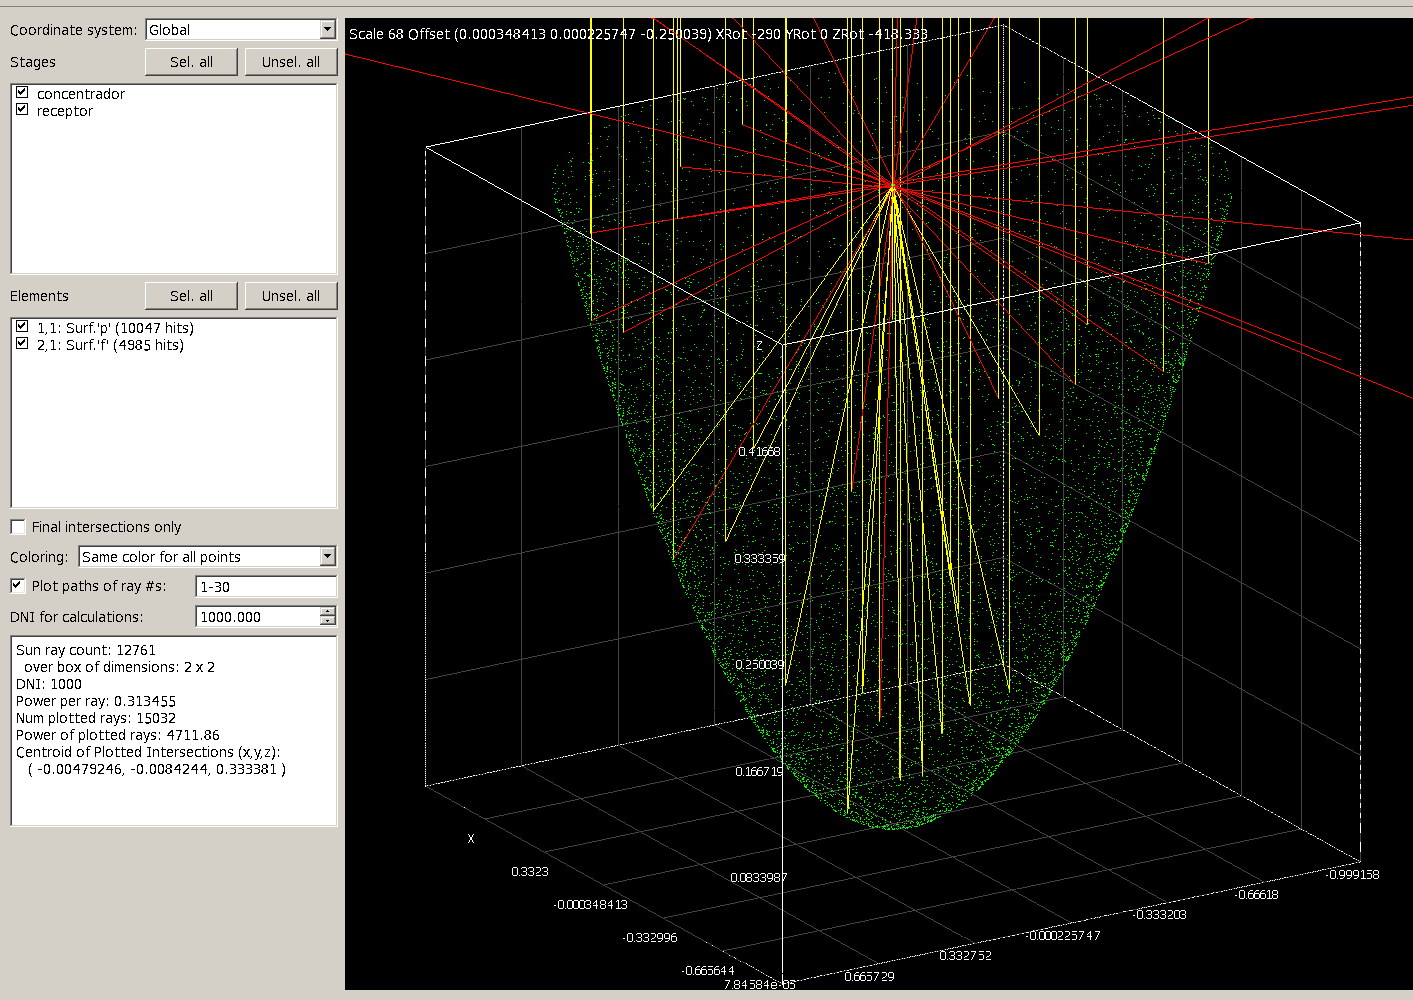
\includegraphics[width=1.0\textwidth]{figures/intersecciones}
  \caption{\label{fig:inter}  Sección de \emph{Intersections} de resultados en SolTrace.}
\end{figure}


En la sección de \emph{Flux Maps} se puede seleccionar la sección de interes a visualizar. En este casao unicamente tenemos un elemento. En esta sección podemos indicar el tamaño de la malla, que por default es de 20$\times$20. Existe también una sección para exportar los datos que nos genera dos archivos uno de con la extensión de ``.tec'' y ``.flx'', el primero se un archivo de datos que contiene la coordenadas y el valor de intensidad que le corresponde. El segundo archivo es la misma información pero en un arreglo matricial. Y por último, existe una sección en donde se muestran un resumen de la simulación. La Figura~\ref{fig:flux} muestra la pestaña de \emph{Contour Plot} en donde se observa la distribución de flujo, la pestaña de \emph{Surface Plot} nos muestra la misma información en 3D.

\begin{figure}[ht]
  \centering
  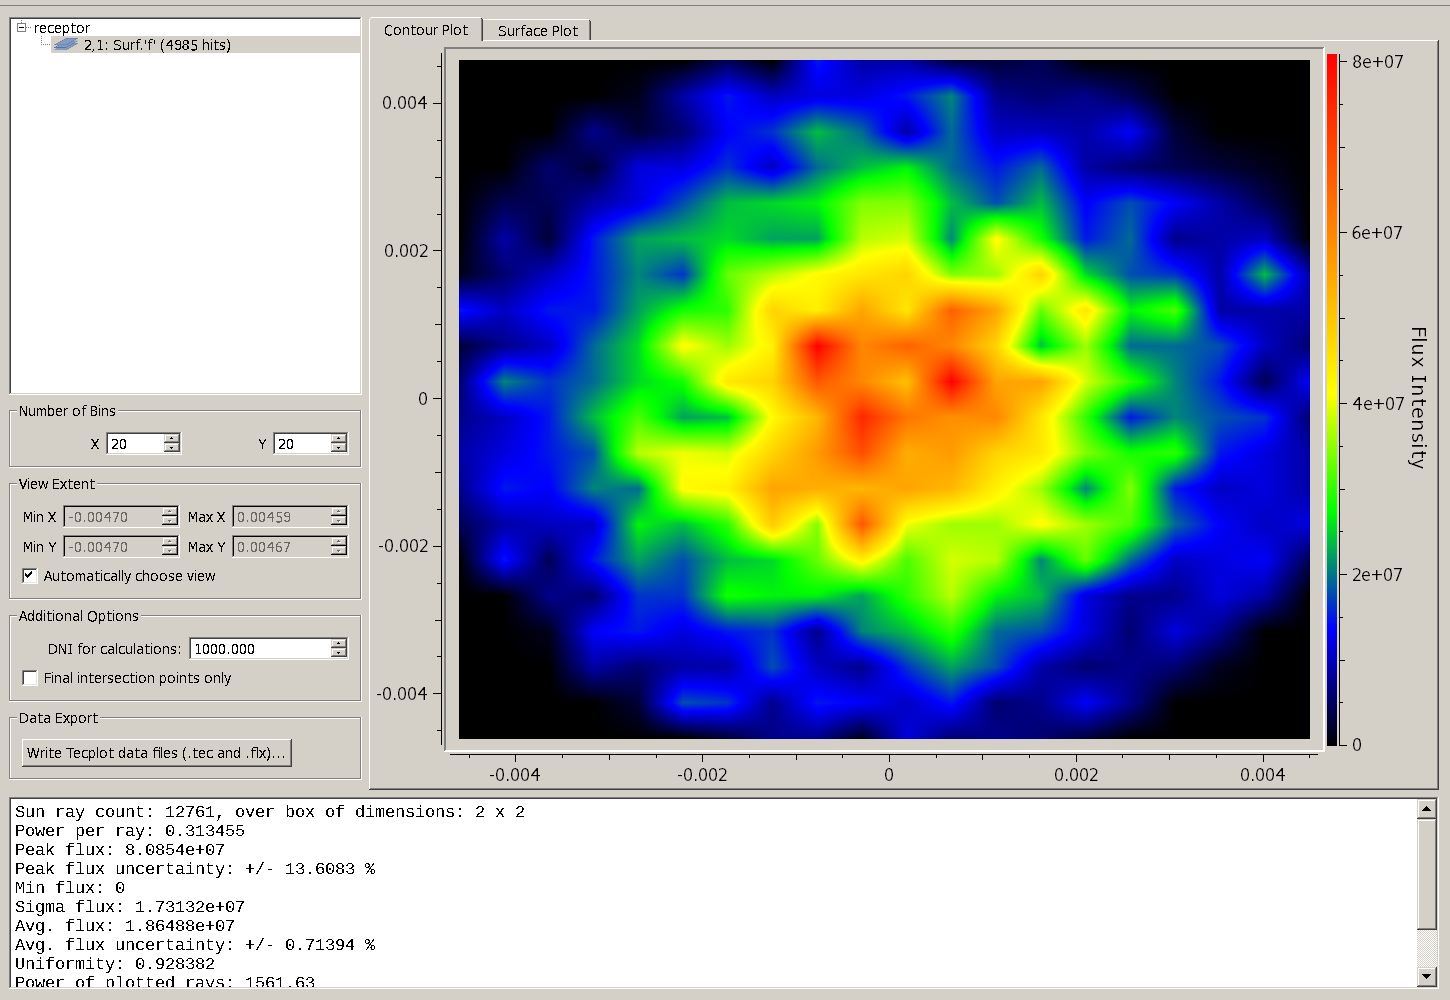
\includegraphics[width=1.0\textwidth]{figures/flux}
  \caption{\label{fig:flux} Distribución de flujo en el receptor.}
\end{figure}

La sección de \emph{Ray Data} nos permite explortar la información del trazado de rayos en un archivo ``.csv''.

Por último realizaremos un trazado de rayos con 7 millones de rayos, mismo que exportaremos con una malla de 35$\times$35.

\begin{figure}[ht]
  \centering
  \subfigure[]{
    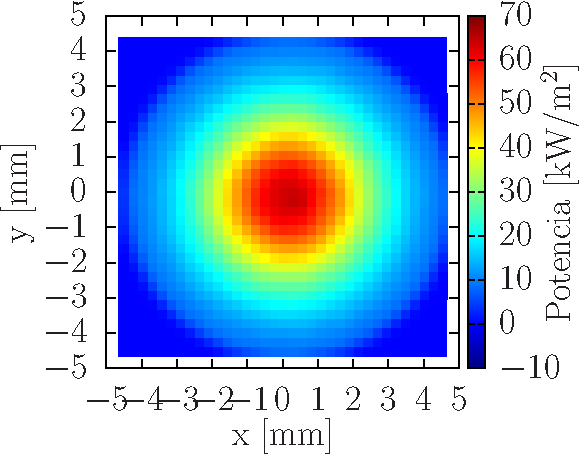
\includegraphics[width=0.45\textwidth]{figures/flux_disco}}
  \subfigure[]{
  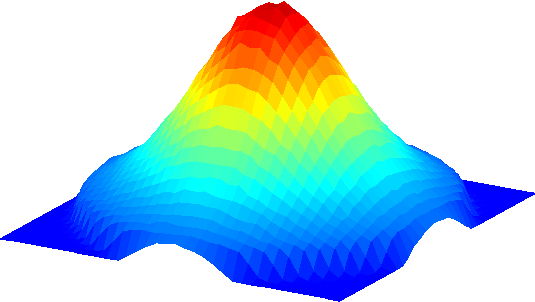
\includegraphics[width=0.5\textwidth]{figures/receptor3d}}
  \caption{\label{fig:fluxDisco} Flujo en el receptor.}
\end{figure}



%%% Local Variables: ***
%%% mode: latex ***
%%% TeX-master: "taller.tex" ***
%%% End: ***
